\input{preamble.tex}

% --------------------------------------------------------------------
% ---- ENTER YOUR PROJECT DETAILS BELOW

\title{Weather Data Analysis --- Indian Cities (2000--2024)}

\author{
    \small Rishabh Das \and
    \small Aakarsh Joshi \and
    \small Raghav Pareek \and
    \small Hire Sakshi
    }

\rhead{Group 8}

% --------------------------------------------------------------------


% --------------------------------------------------------------------
% ---- DO NOT CHANGE THIS BLOCK OF CODE
\begin{document}
\maketitle
% --------------------------------------------------------------------



% --------------------------------------------------------------------
% ---- WRITE YOUR REPORT BELOW

\section{Introduction}
% TODO: to be filled by team

\section{Related Work}
% TODO: to be filled by team

\section{Our Contribution}
% TODO: to be filled by team

\section{Methods}

\subsection{Data}
The dataset used in this project is the NOAA Global Summary of the Day (GSOD),
a publicly available database that records daily weather observations from stations
around the world. Data was collected for four Indian cities --- Mumbai, Delhi,
Dehradun, and Jodhpur --- covering 25 years from 2000 to 2024.
Each city has a unique NOAA station ID: Mumbai (43003099999), Delhi (42182099999),
Dehradun (42110099999), and Jodhpur (42339099999).
Variables available include mean temperature, maximum and minimum temperature,
dew point, precipitation, wind speed, visibility, and pressure.

\subsection{Data Collection}
Data was downloaded directly from NOAA's servers using Python with no manual
steps involved. For each city, yearly CSV files were fetched from the following URL:

\begin{center}
\texttt{https://www.ncei.noaa.gov/data/global-summary-of-the-day/access/\{year\}/\{station\_id\}.csv}
\end{center}

A plain \texttt{requests.get()} call kept returning HTTP 503 errors because NOAA's
CDN blocks automated requests. The fix was to use a \texttt{requests.Session} with
browser-like headers (Chrome User-Agent, Accept-Language, Referer), along with retry
logic that waits and tries again if the server returns a 503 or 429 response.
A small random delay between requests was also added to avoid triggering rate limits.
To speed up the download, \texttt{ThreadPoolExecutor} was used to fetch 3 years
simultaneously instead of one by one.

The download code is split into one file per city inside the \texttt{raw\_data/} folder
(\texttt{mumbai\_raw.py}, \texttt{delhi\_raw.py}, \texttt{dehradun\_raw.py},
\texttt{jodhpur\_raw.py}). Each file exposes a single \texttt{get\_raw\_data()} function
that returns a combined dataframe for that city covering all 25 years.
To avoid re-downloading every time the code is run, the downloaded data is saved
as a \texttt{.nc} (NetCDF) file in \texttt{raw\_data/nc\_raw/} and loaded from
there on subsequent runs.

\subsection{Data Cleaning}
Raw NOAA data has several issues that need to be fixed before any analysis.
The cleaning pipeline is in the \texttt{cleaned\_data/} folder, with one file
per city. Each file imports raw data from the corresponding raw file, runs
the cleaning steps below in order, and saves the result as a \texttt{.nc} file
in \texttt{cleaned\_data/nc\_cleaned/}.

\begin{enumerate}

    \item \textbf{Date parsing.}
    The \texttt{DATE} column was parsed to datetime format and rows with
    unreadable dates were dropped. \texttt{YEAR} and \texttt{MONTH} columns
    were extracted for use in grouping later.

    \item \textbf{Replace fill values with NaN.}
    NOAA does not use NaN for missing data. Instead it uses large placeholder
    numbers --- 9999.9 for temperature, 99.99 for precipitation, 999.9 for
    wind and visibility. These were identified and replaced with NaN before
    any other step, otherwise they appear as real observations and break
    all statistics.

    \item \textbf{Remove duplicate dates.}
    Some years had more than one row for the same date. Duplicates were
    removed by keeping the first occurrence.

    \item \textbf{Unit conversion.}
    NOAA stores data in imperial units. All variables were converted to
    metric --- Fahrenheit to Celsius, inches to mm, knots to m/s, and miles
    to km. Columns were renamed to reflect the new units
    (\texttt{TEMP\_C}, \texttt{PRCP\_MM}, \texttt{WDSP\_MS} etc.).

    \item \textbf{Remove physically impossible values.}
    After unit conversion, a physical plausibility check was applied.
    Temperature above 60\textdegree C or below -90\textdegree C goes beyond
    any recorded Earth extreme. Negative rainfall or wind speed cannot exist.
    Rainfall above 2000mm in a single day exceeds the world record.
    Days where MAX temperature is lower than MIN are recording errors.
    Dew point above air temperature is physically impossible.
    All such values were set to NaN rather than corrected, since there is
    no reliable way to know what the actual reading should have been.

    \item \textbf{Anomaly detection.}
    A robust z-score was computed per variable per month using the median
    and MAD (Median Absolute Deviation) rather than mean and standard
    deviation. This choice is important --- using mean and SD on weather
    data is problematic because a real extreme event like a flood inflates
    the mean, making the event look less unusual than it actually is.
    The formula used is:
    \begin{align}
        z = \frac{0.6745 \times (x - \tilde{x})}{\mathrm{MAD}}
        \label{eq:zscore}
    \end{align}
    where $\tilde{x}$ is the monthly median and MAD is the median absolute
    deviation for that month. Values with $|z| > 3.5$ were flagged as
    anomalies and set to NaN, \emph{except} for rows corresponding to known
    historical extreme events (such as the 2005 Mumbai floods and the 2013
    Uttarakhand cloudbursts) which were protected from removal.

    \item \textbf{Select output columns.}
    The final dataframe keeps only the columns needed for analysis:
    DATE, CITY, YEAR, MONTH, TEMP\_C, MAX\_C, MIN\_C, DEWP\_C, PRCP\_MM,
    WDSP\_MS, MXSPD\_MS, GUST\_MS, and FRSHTT. Everything else is dropped.

\end{enumerate}

\section{Results}

\subsection{Data Quality Report}

After downloading and cleaning the data, a data quality report was produced
to understand how reliable the data is across all four cities.
The report consists of two figures generated by \texttt{data\_quality\_report.py}.

Figure~\ref{fig:missing} shows one heatmap per city, where each cell represents
the percentage of values that were missing (either empty or set to the NOAA
fill value) for a given variable in a given year. This revealed that GUST and
SLP are almost entirely missing across all cities and all years. This is not
a data error --- Indian IMD stations simply do not transmit these variables
to NOAA's GSOD database. Core variables like TEMP, MAX, MIN, and WDSP are
well recorded with under 2\% missing for all cities.

\begin{figure}[tbp]
    \begin{center}
        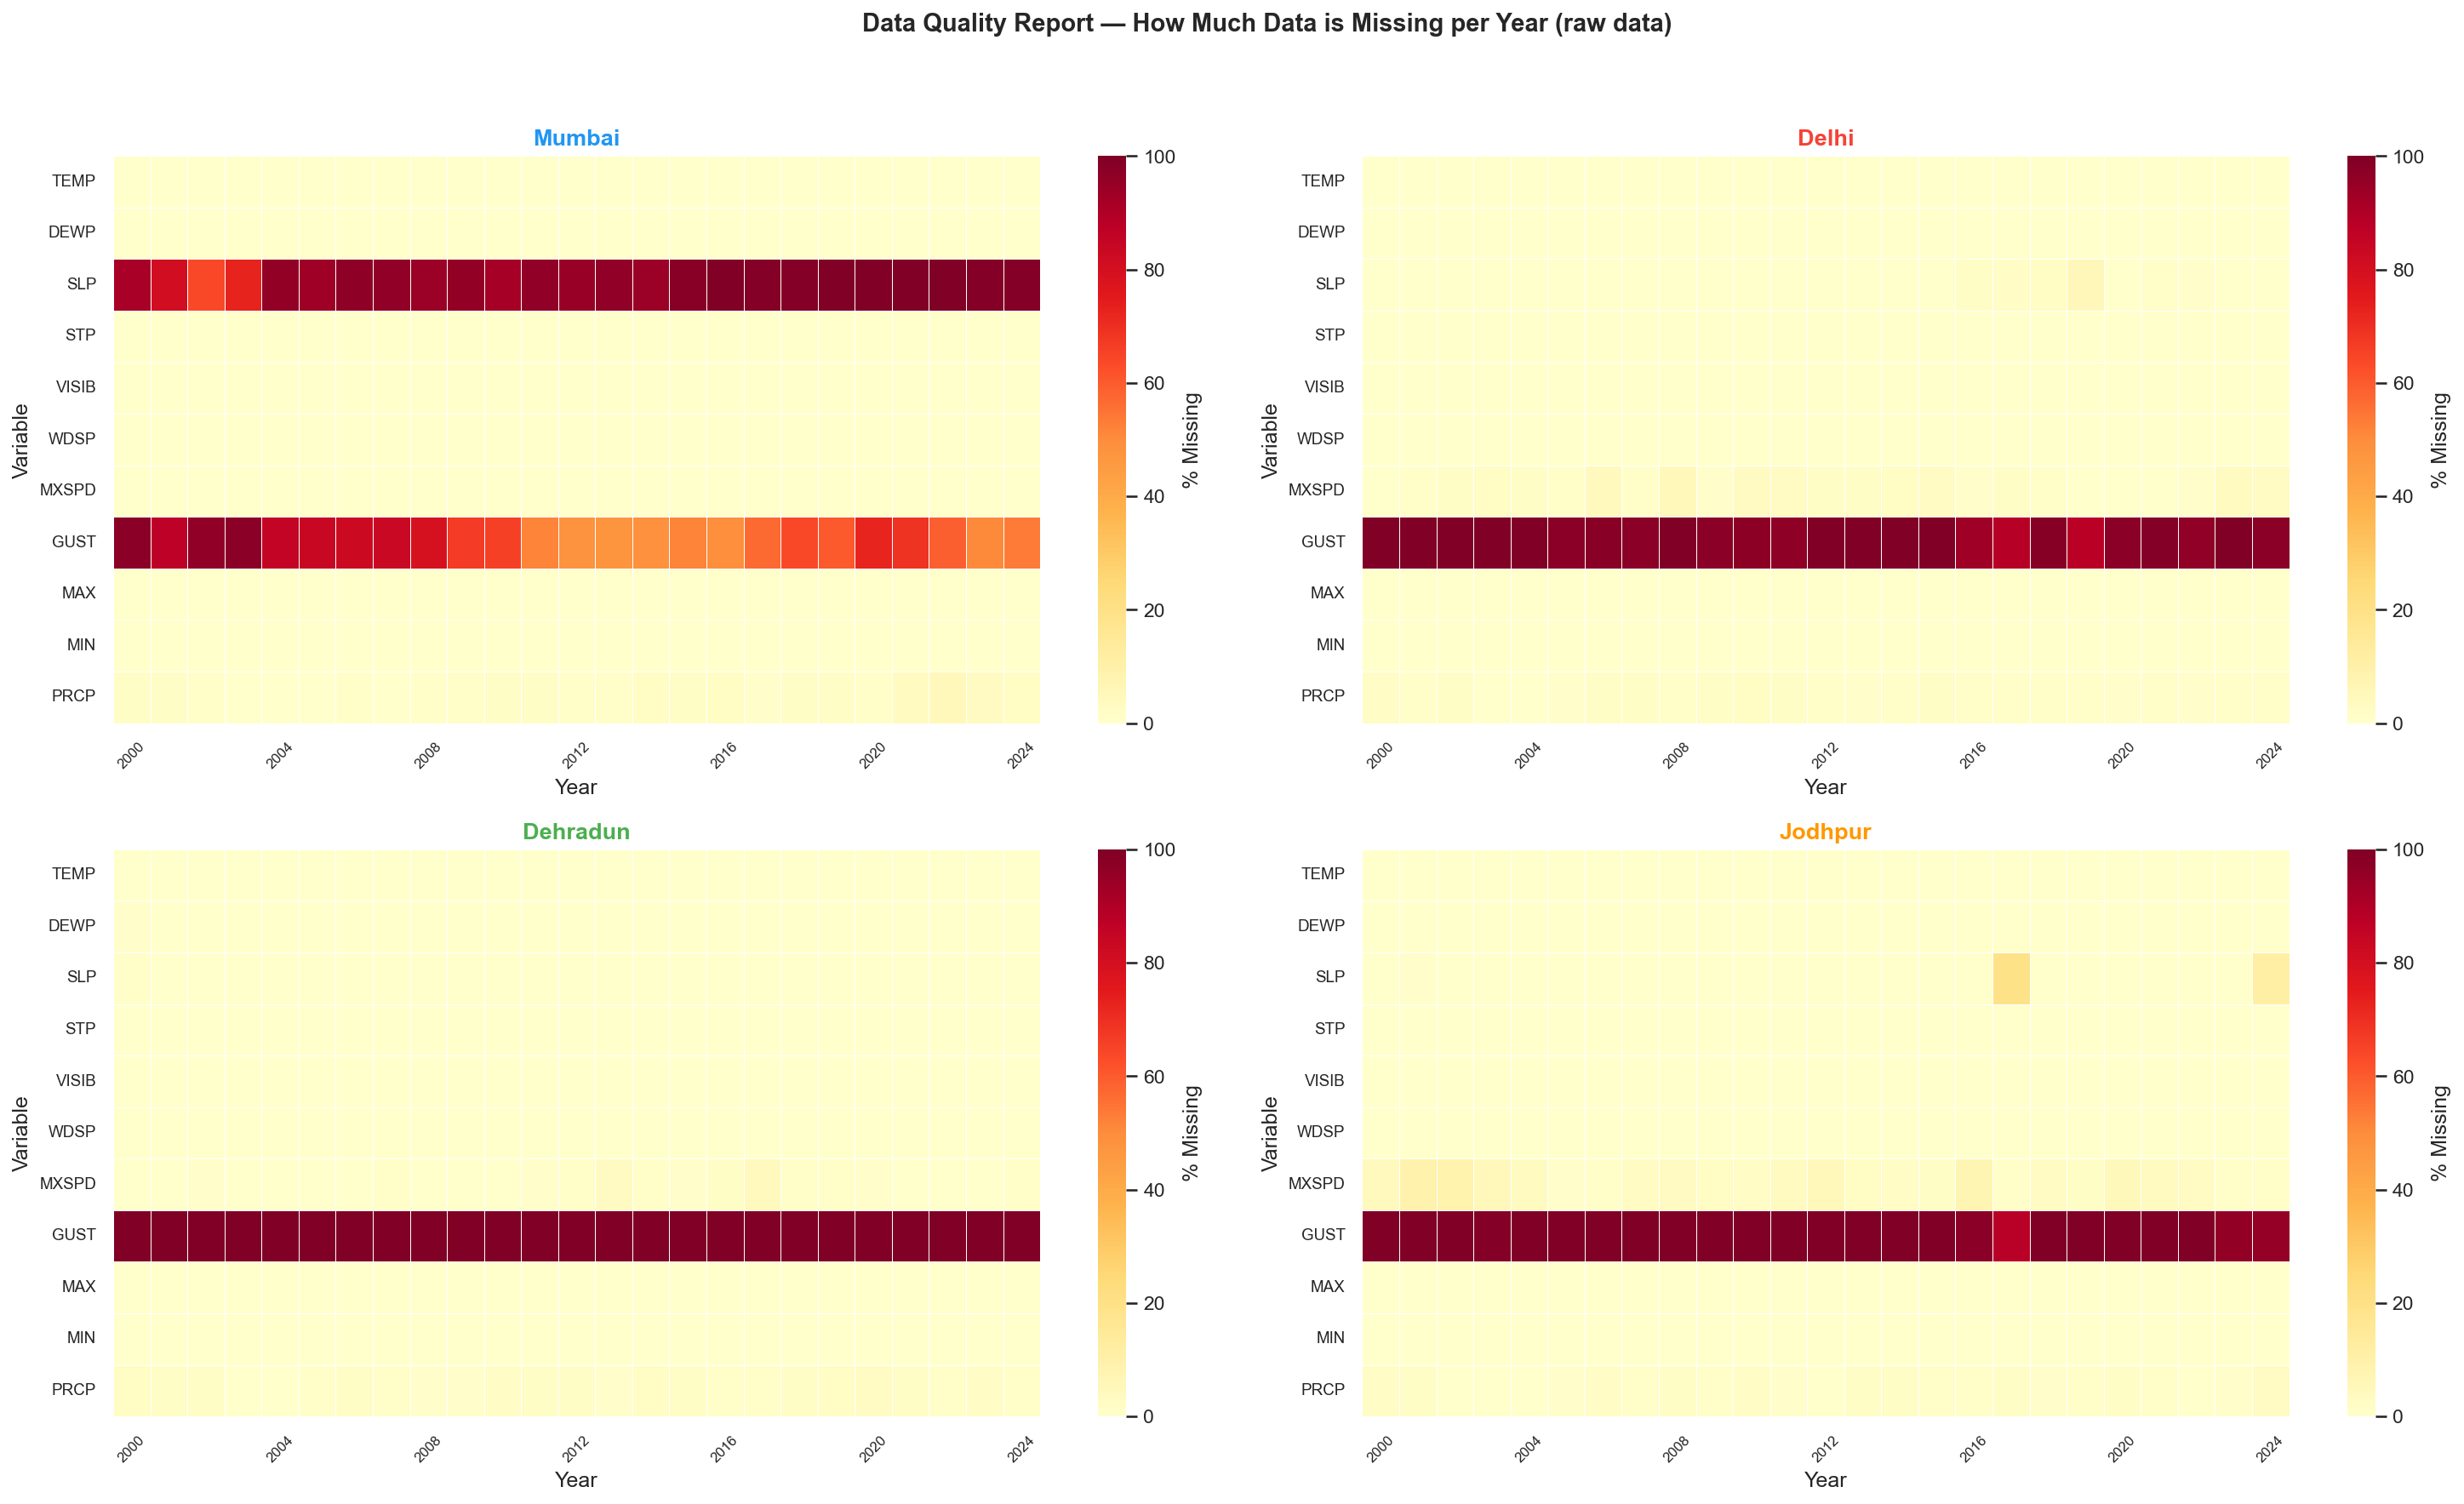
\includegraphics[width=\textwidth]{./figures/data_quality_missing.png}
        \caption{Missing data percentage per variable per year for each city (raw data).
        Dark red cells indicate variables that are almost entirely missing.
        GUST and SLP are missing across all cities because Indian stations
        do not transmit these to NOAA's GSOD database.}
        \label{fig:missing}
    \end{center}
\end{figure}

Figure~\ref{fig:stats} shows four panels. The first panel shows how many days
were recorded per year per city, with a reference line at 365. Dehradun shows
some years with noticeably fewer observations, especially around 2000, consistent
with smaller inland stations having occasional reporting gaps. The second panel
shows the count of NaN values per variable per city in the cleaned data.
The third panel is a summary statistics table showing mean, standard deviation,
min, max, and median for temperature and precipitation per city.
The fourth panel shows how many fill values were found and replaced per city ---
Mumbai had the highest count at 14,957 (mostly from GUST and SLP columns),
while Delhi had 9,208 and Jodhpur had 9,442.

\begin{figure}[tbp]
    \begin{center}
        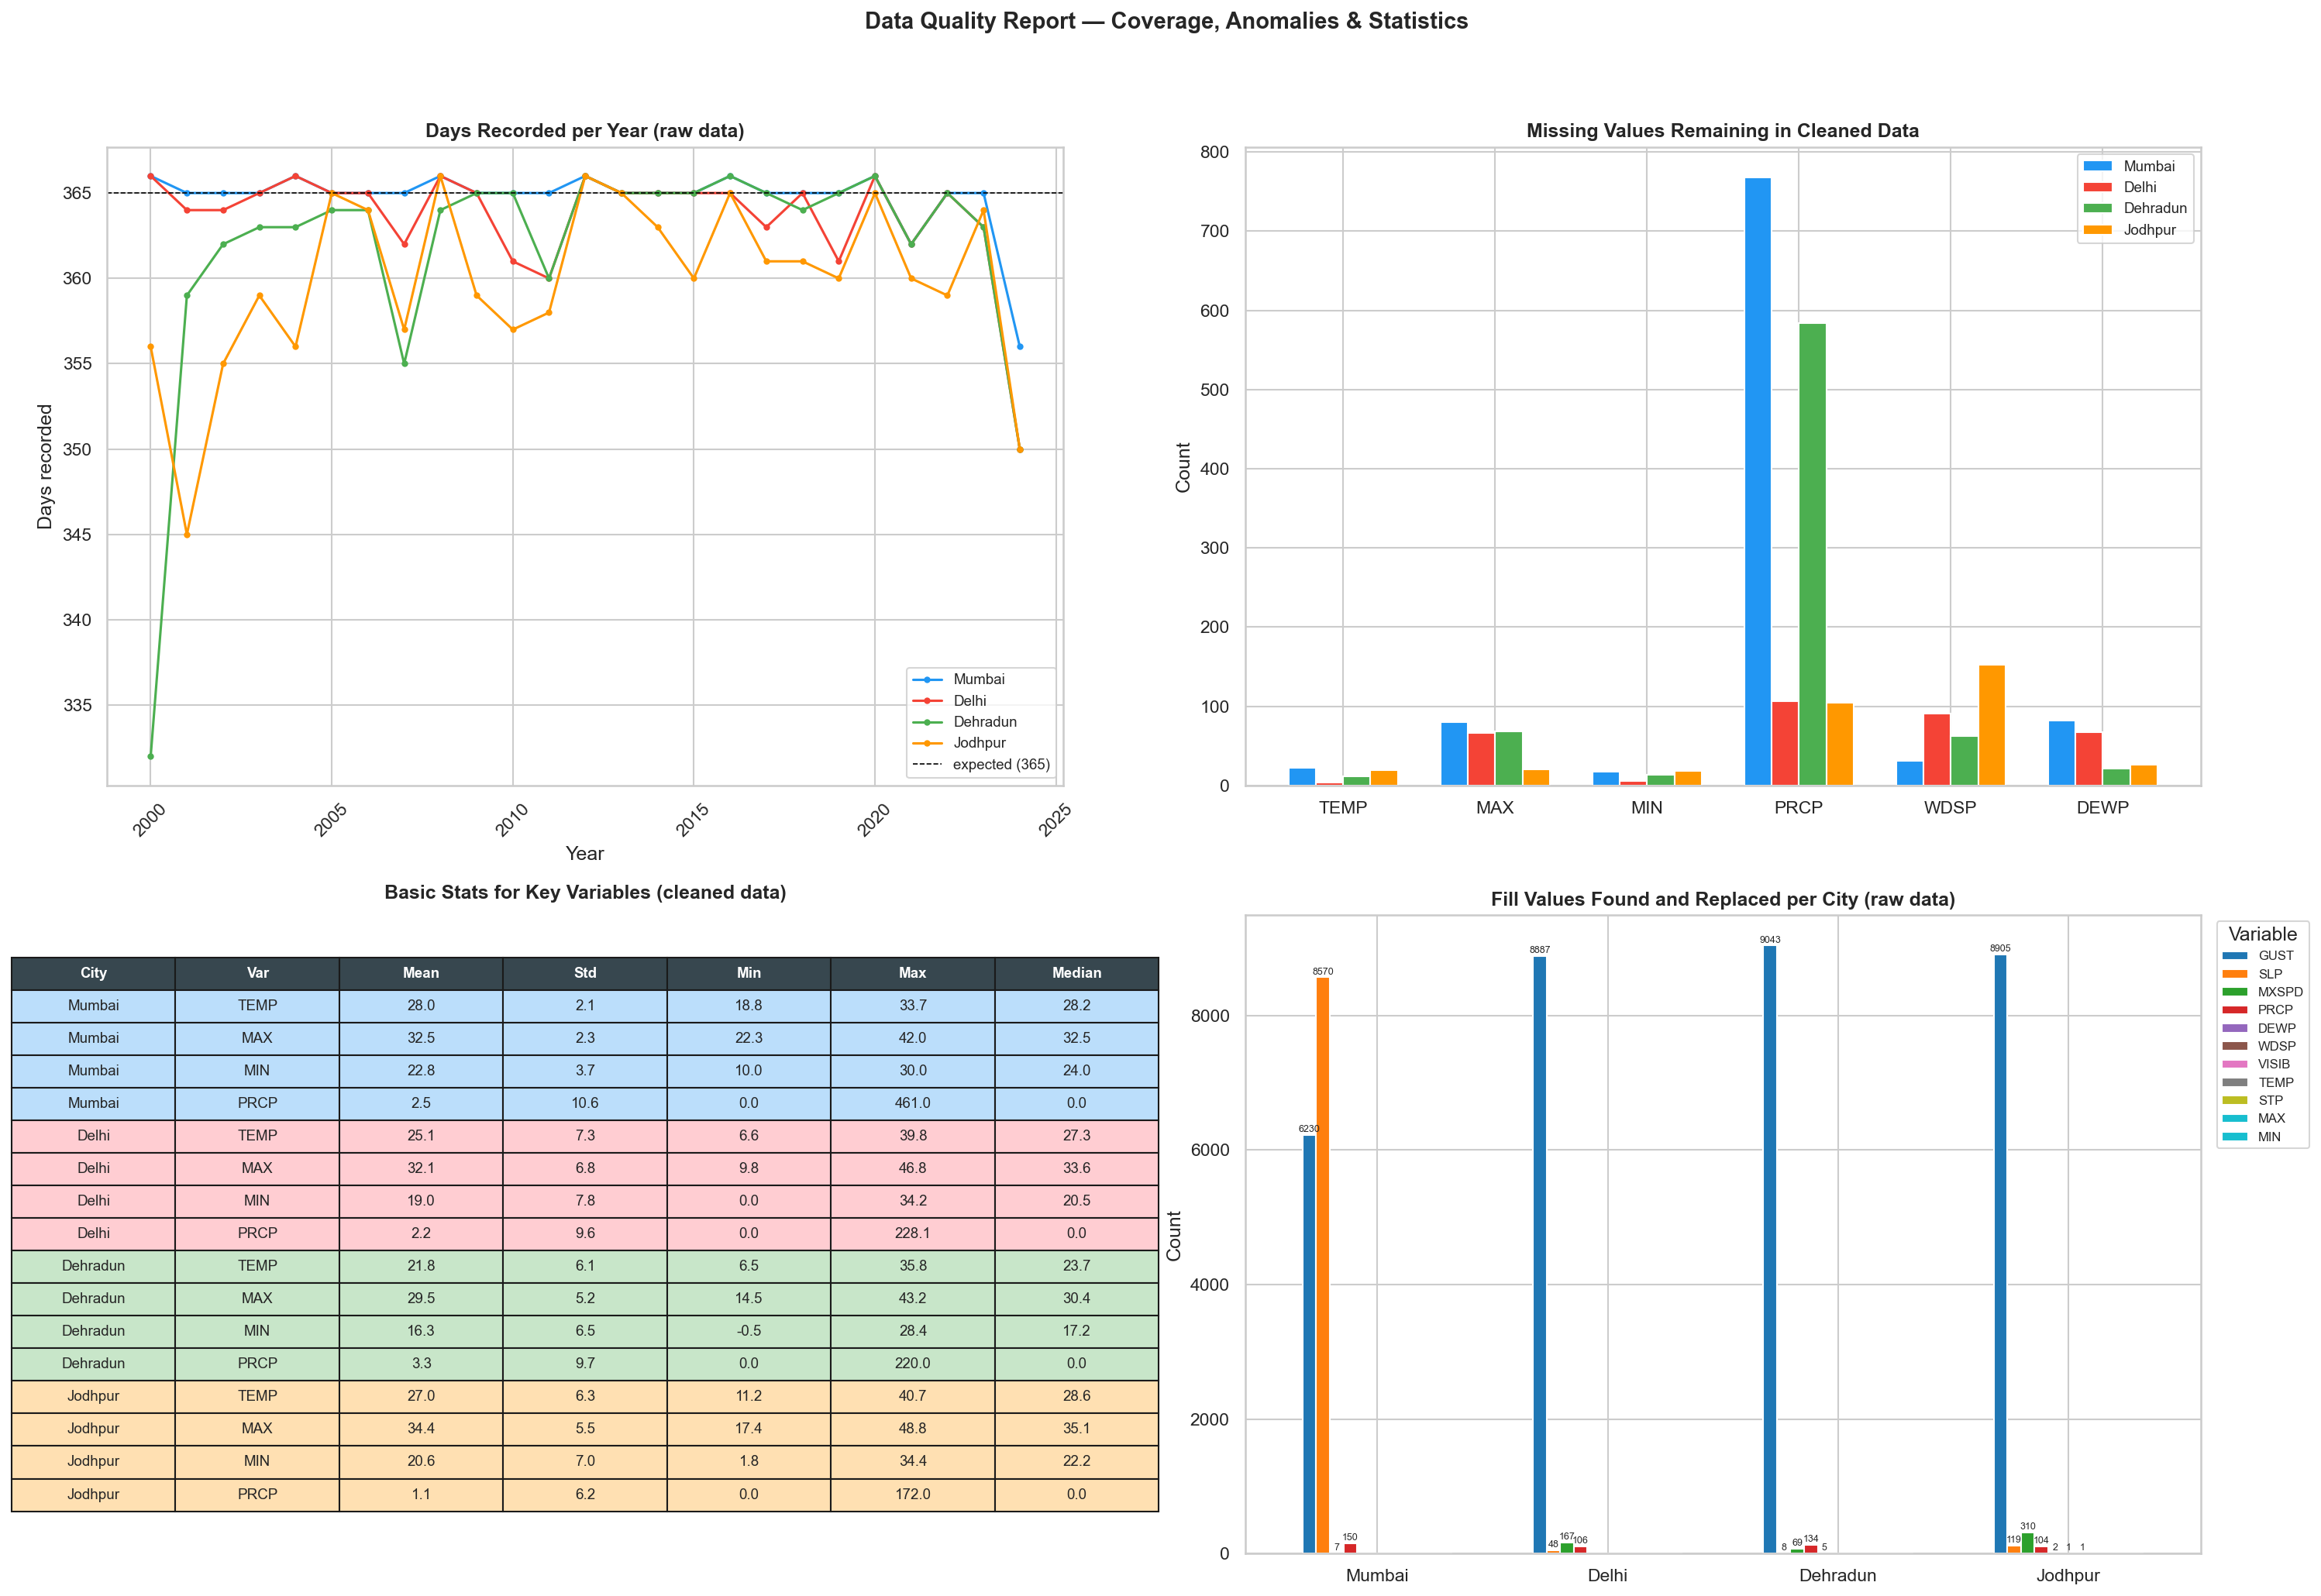
\includegraphics[width=\textwidth]{./figures/data_quality_stats.png}
        \caption{Data quality summary: record coverage per year, NaN counts,
        descriptive statistics, and fill value replacement counts per city.}
        \label{fig:stats}
    \end{center}
\end{figure}

\subsection{Seasonal Patterns}

\begin{figure}[tbp]
    \begin{center}
        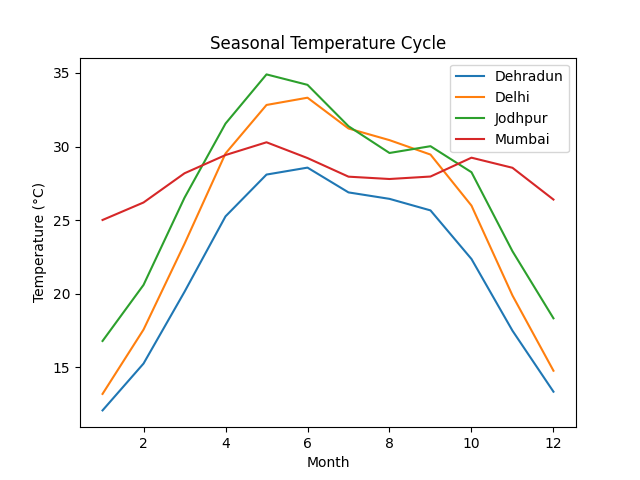
\includegraphics[width=\textwidth]{./figures/temp_seasonality.png}
        \caption{Monthly temperature seasonality across cities.}
        \label{fig:temp_seasonality}
    \end{center}
\end{figure}

\begin{figure}[tbp]
    \begin{center}
        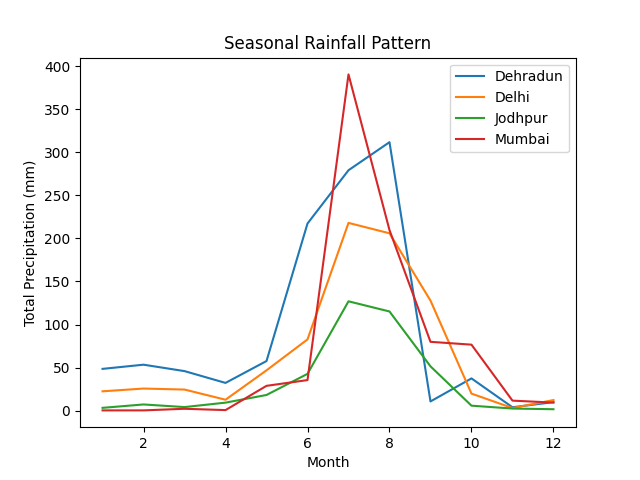
\includegraphics[width=\textwidth]{./figures/rainfall_seasonality.png}
        \caption{Monthly rainfall seasonality across cities.}
        \label{fig:rainfall_seasonality}
    \end{center}
\end{figure}

The seasonal patterns reveal clear climatic differences across cities
(Figures~\ref{fig:temp_seasonality} and~\ref{fig:rainfall_seasonality}).
Mumbai stands out with consistently high humidity and relatively stable temperatures,
showing minimal variation due to its coastal influence.
In contrast, Delhi and Jodhpur exhibit sharper temperature fluctuations,
with very hot summers and cooler winters, indicating a more continental climate.
Rainfall patterns further differentiate the cities: Mumbai experiences a pronounced
monsoon peak, while Dehradun shows significant but slightly more distributed rainfall.
Jodhpur, being more arid, records comparatively lower rainfall overall.
These variations highlight how geography influences seasonal weather behaviour
across regions.

\subsection{Yearly (Interannual) Analysis}

\begin{figure}[tbp]
    \begin{center}
        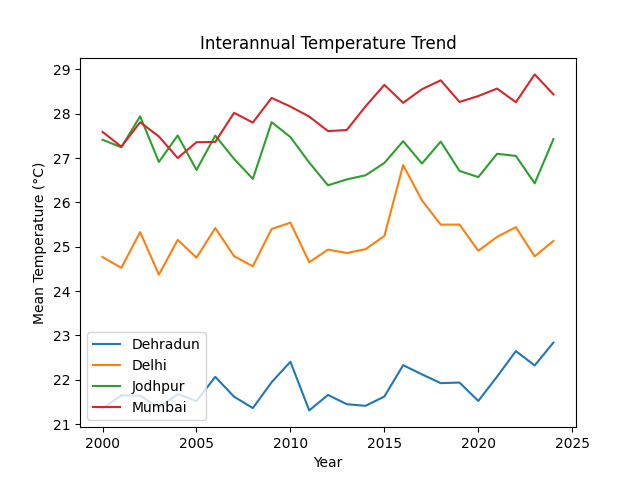
\includegraphics[width=\textwidth]{./figures/temp_trend.png}
        \caption{Interannual temperature trends across cities (2000--2024).}
        \label{fig:temp_trend}
    \end{center}
\end{figure}

\begin{figure}[tbp]
    \begin{center}
        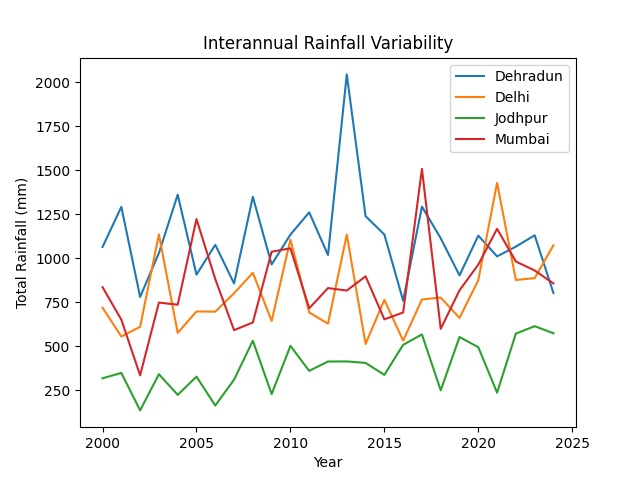
\includegraphics[width=\textwidth]{./figures/rainfall_trend.png}
        \caption{Interannual rainfall trends across cities (2000--2024).}
        \label{fig:rainfall_trend}
    \end{center}
\end{figure}

The interannual temperature trends suggest gradual changes with distinct city-wise
behaviour (Figures~\ref{fig:temp_trend} and~\ref{fig:rainfall_trend}).
Mumbai consistently records the highest average temperatures with a slight upward
trend, indicating relatively stable yet warming conditions over time.
Jodhpur also maintains higher temperatures but shows more variability compared to Mumbai.
Delhi demonstrates moderate temperatures with noticeable fluctuations, possibly
reflecting sensitivity to yearly climatic variations.
Meanwhile, Dehradun remains the coolest among the four, with smaller variations
but a subtle increasing trend in recent years.
Overall, while all cities show some degree of warming, the rate and variability
differ, emphasising unique local climate dynamics.

\subsection{Variability}

\begin{figure}[tbp]
    \begin{center}
        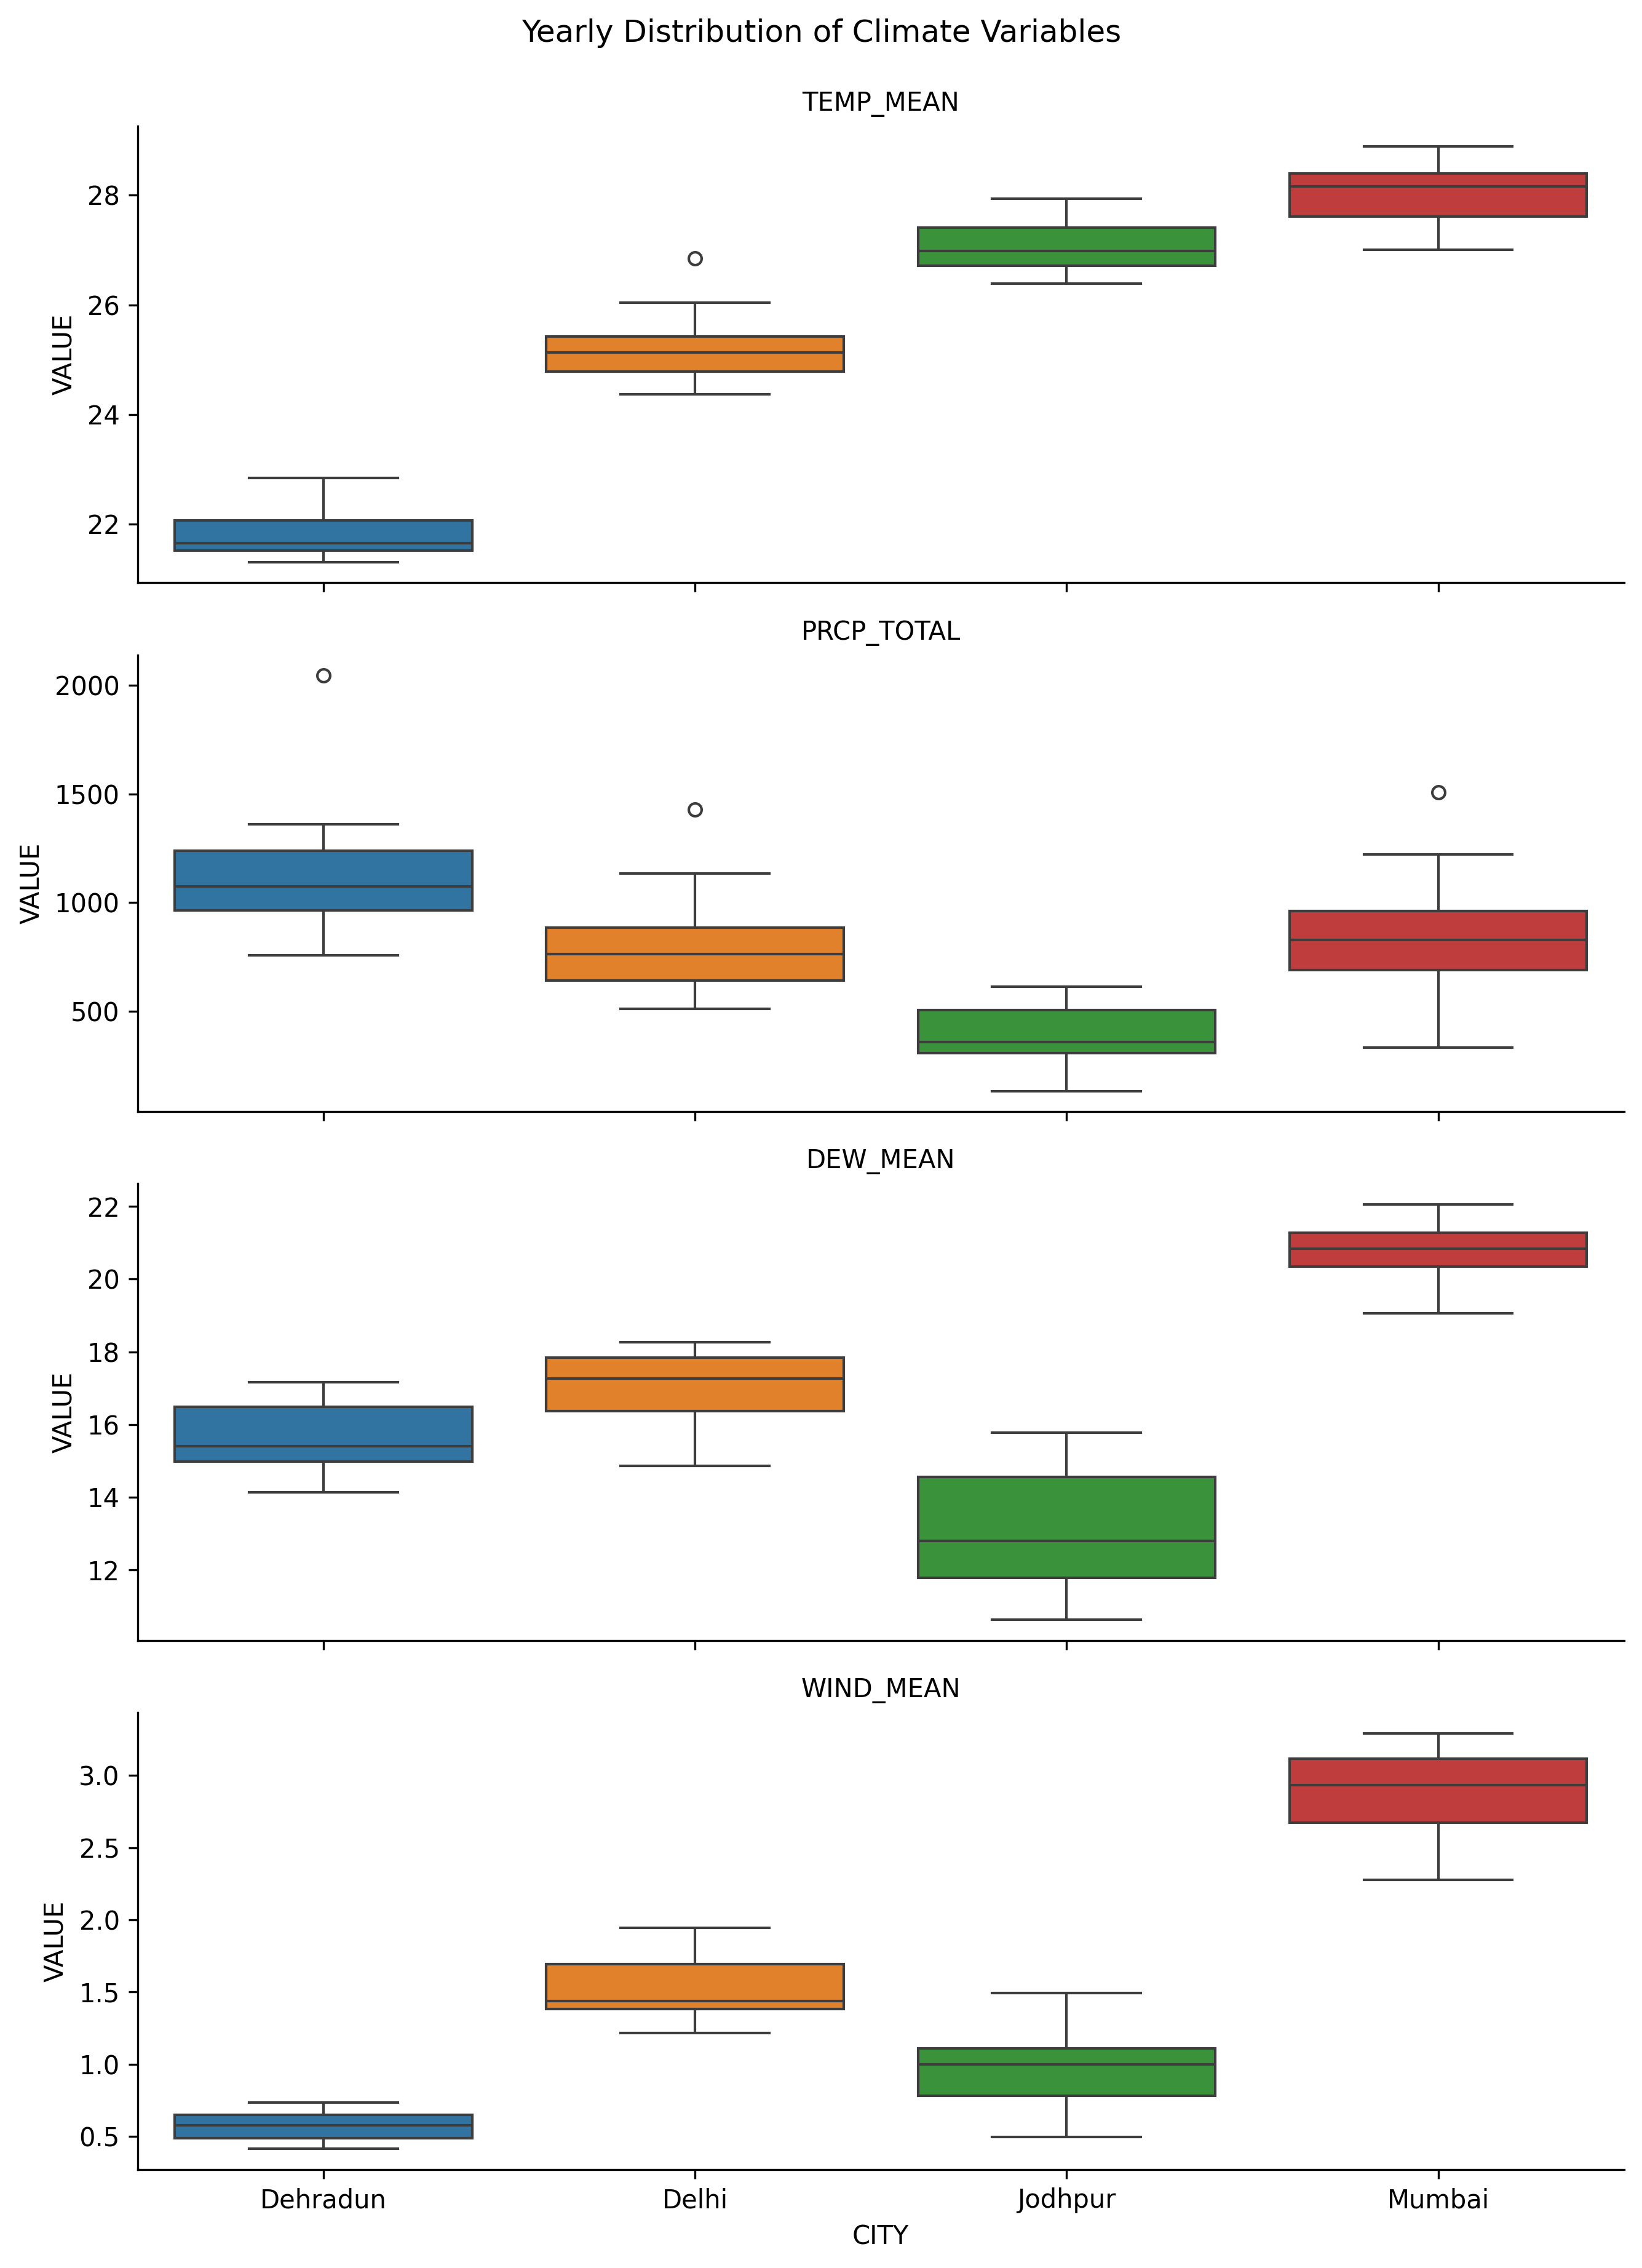
\includegraphics[width=\textwidth]{./figures/yearly_variability_box.png}
        \caption{Year-to-year variability across cities shown as box plots.}
        \label{fig:variability_box}
    \end{center}
\end{figure}

\begin{figure}[tbp]
    \begin{center}
        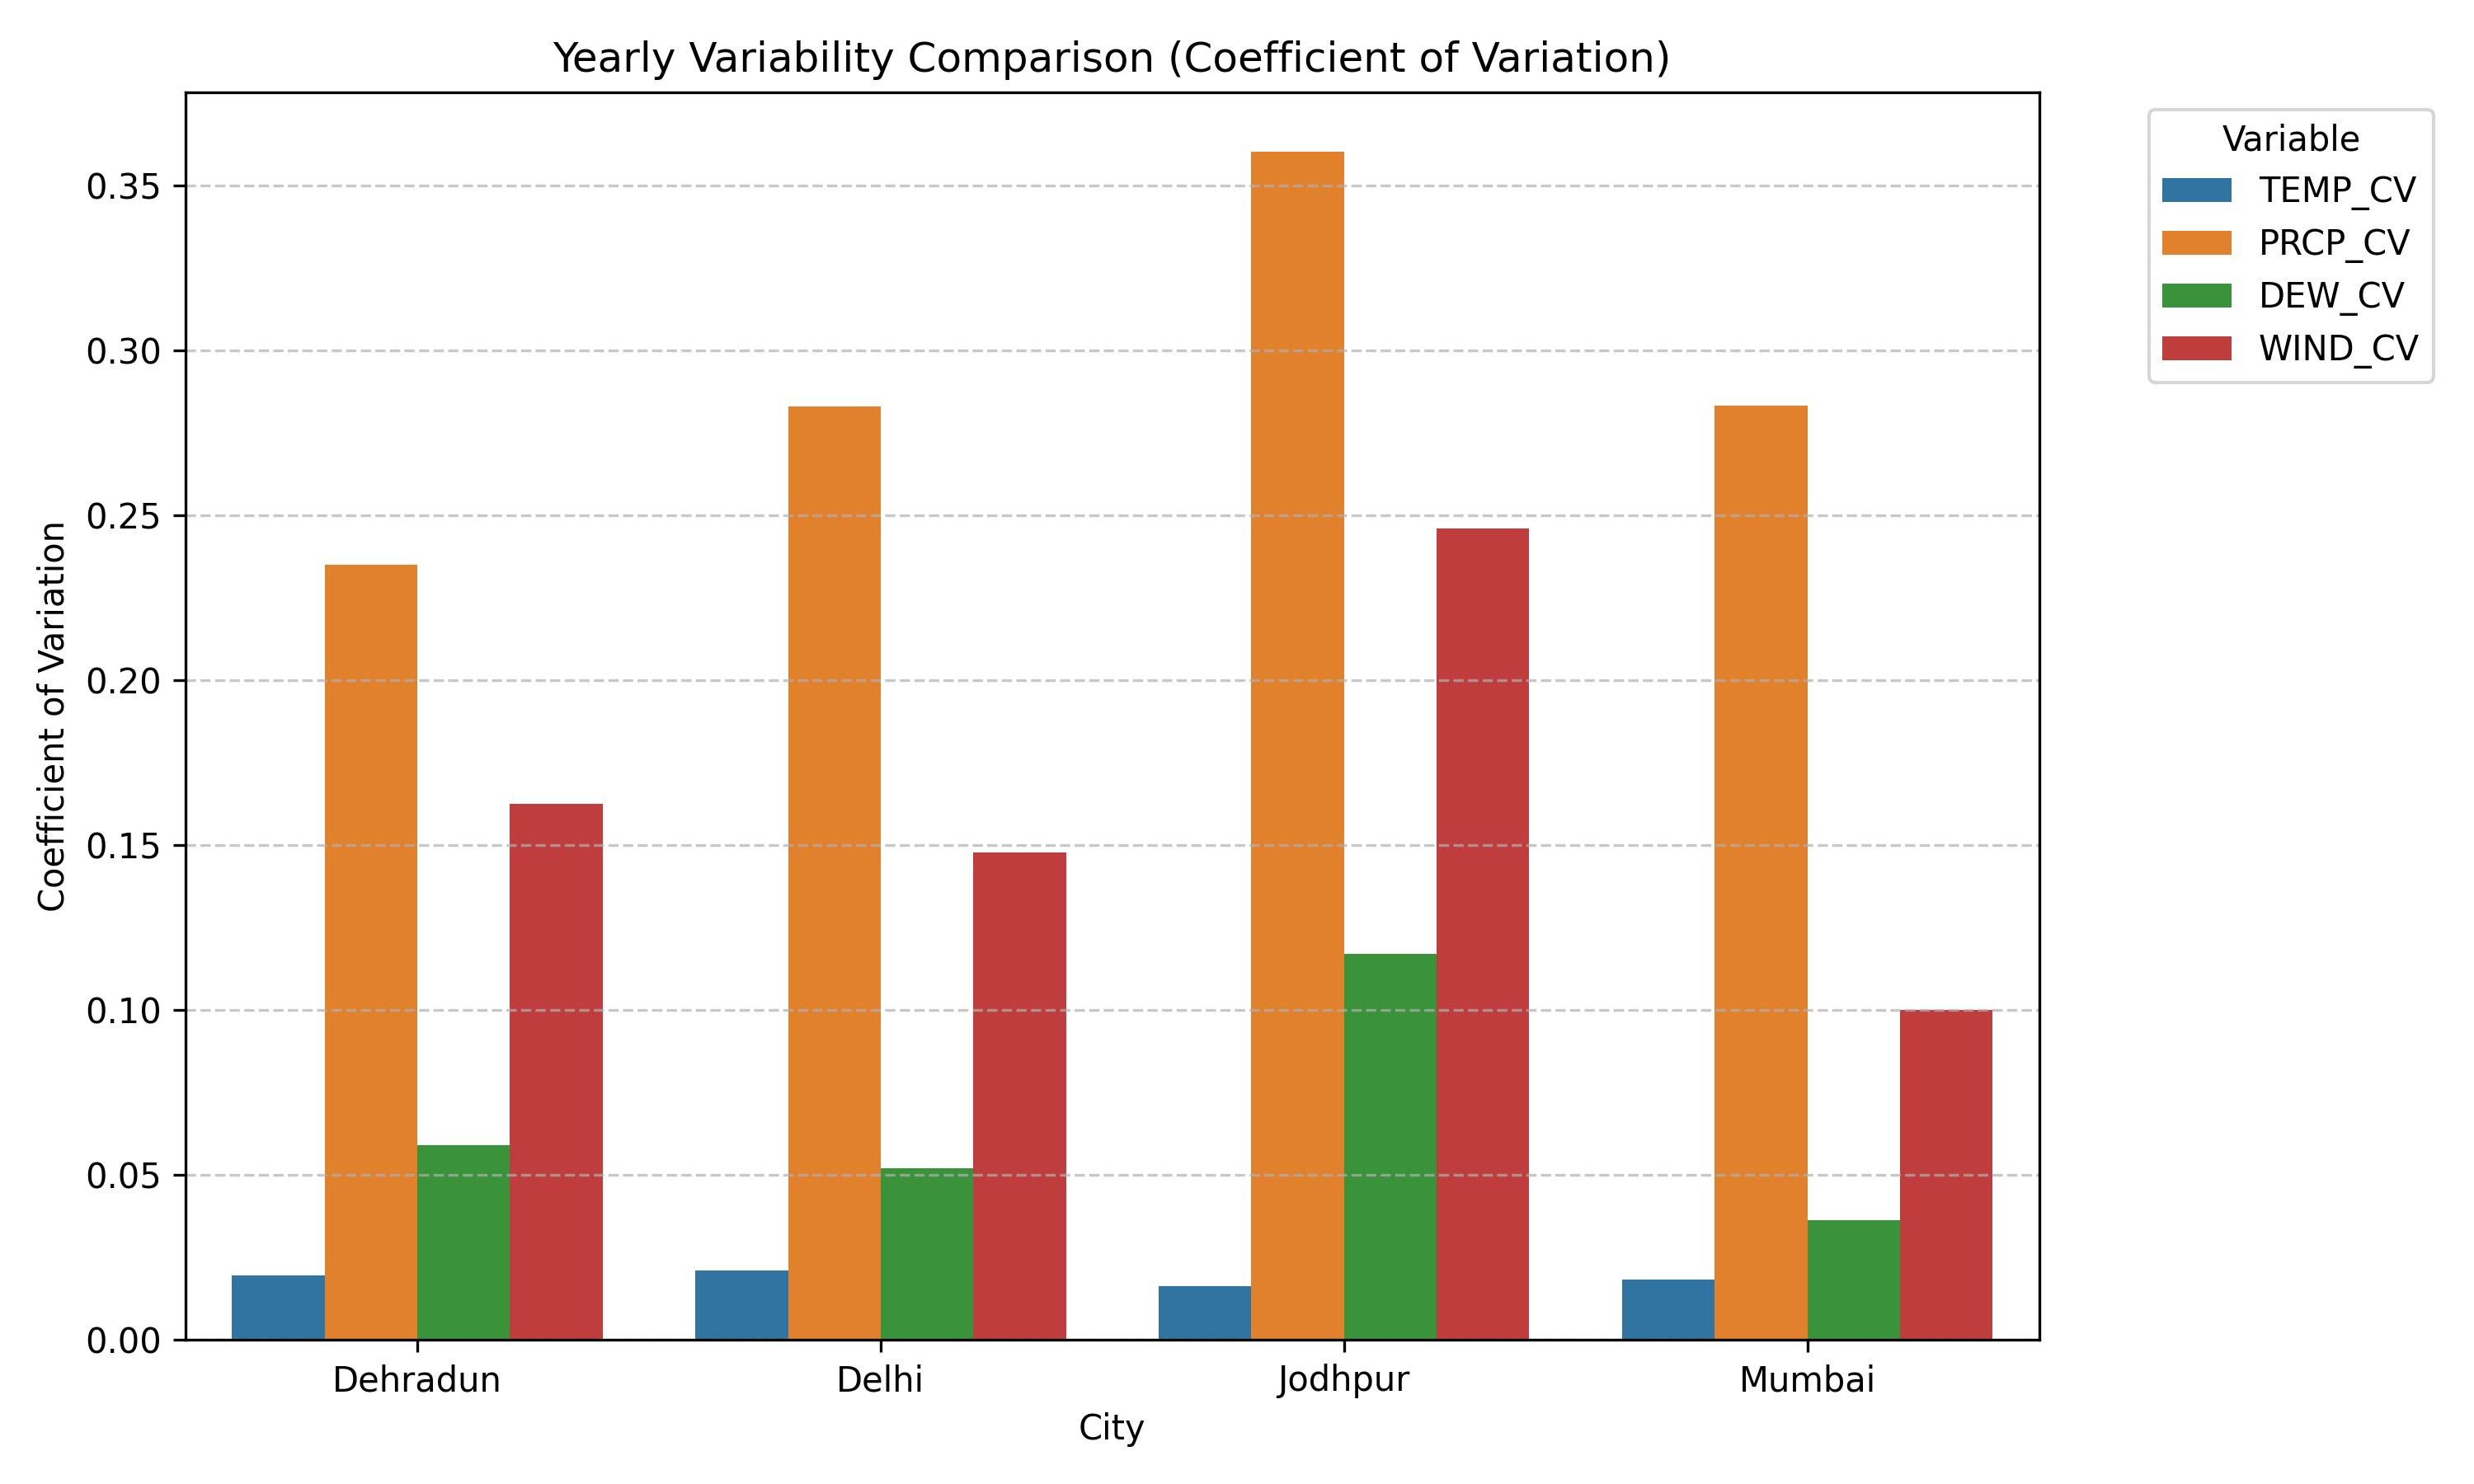
\includegraphics[width=\textwidth]{./figures/yearly_variability_bar.png}
        \caption{Year-to-year variability across cities shown as bar charts.}
        \label{fig:variability_bar}
    \end{center}
\end{figure}

The data reveals distinct climate patterns across the four cities, with precipitation
showing the highest variability overall
(Figures~\ref{fig:variability_box} and~\ref{fig:variability_bar}).
Jodhpur stands out with the most significant fluctuations in rainfall (\texttt{PRCP\_CV})
and wind speed, while maintaining a relatively high mean temperature.
In contrast, Mumbai experiences the highest average temperatures, dew points, and
wind speeds, yet shows the lowest variability in wind, suggesting a more consistent
coastal breeze.
Delhi demonstrates moderate variability across most metrics, with a temperature mean
that sits between the cooler Dehradun and the hotter southern and western cities.
Dehradun remains the coolest of the group with the lowest average wind speeds,
though its rainfall variability remains quite high, nearly matching that of Delhi
and Mumbai.

\subsection{Humidity Analysis}

\begin{figure}[tbp]
    \begin{center}
        \includegraphics[width=\textwidth]{./figures/humidity_comparitive_static.png}
        \caption{Comparative humidity analysis across cities, showing the gap
        between temperature and dew point as a proxy for atmospheric moisture.}
        \label{fig:humidity}
    \end{center}
\end{figure}

Figure~\ref{fig:humidity} illustrates that Mumbai shows higher humidity than
the other cities primarily due to its coastal location along the Arabian Sea.
The graph shows a consistently smaller gap between temperature and dew point,
indicating that the air remains moisture-rich throughout the year.
Unlike inland cities such as Delhi or Jodhpur, where this gap widens during
dry seasons, Mumbai's proximity to the sea ensures a continuous supply of
moisture-laden air.
This results in persistently high humidity levels with less seasonal fluctuation,
especially during the monsoon period when moisture content peaks further.

\section{Conclusion and Outlook}
% TODO: to be filled by team

\section{Acknowledgements}
% TODO: to be filled by team

\section{Author Contributions}
My contribution to this project covered Parts 1, 2, and 3 ---
data collection, data cleaning, and the data quality report.
I wrote the \texttt{raw\_data/} folder with separate download scripts for
each city, handling the NOAA server issues and setting up the \texttt{.nc}
caching system so data only needs to be downloaded once.
I wrote the \texttt{cleaned\_data/} folder with the full cleaning pipeline
per city, including fill value replacement, unit conversion, impossible value
removal, and anomaly detection.
I also wrote \texttt{data\_quality\_report.py} which produces the two
quality figures described in Section~5.1.

\section{Code availability}
The code for this project is available at the following GitHub repository:
\url{https://github.com/Sakshihire06/Weather_Analysis}.
The raw data download scripts are in the \texttt{raw\_data/} folder and
the cleaning scripts are in the \texttt{cleaned\_data/} folder.

% --------------------------------------------------------------------
% ---- DO NOT CHANGE THIS BLOCK OF CODE
\section{References}
\bibliography{refs}
% --------------------------------------------------------------------


\section{Appendix}

\subsection{Additional figures}
% TODO: add any extra figures here if needed

\subsection{Algorithms}
% TODO: add any algorithms here if needed

\subsection{Code snippets}

The function below shows the core of the anomaly detection step used
in the cleaning pipeline.

\begin{minted}[bgcolor=white, fontsize=\small, linenos, frame=none]{python}
for col in ['TEMP_C', 'MAX_C', 'MIN_C', 'PRCP_MM', 'WDSP_MS', 'DEWP_C']:
    monthly_median = df.groupby('MONTH')[col].transform('median')
    monthly_mad    = df.groupby('MONTH')[col].transform(
        lambda x: (x - x.median()).abs().median()
    )
    zscore = np.where(
        monthly_mad > 0,
        0.6745 * (df[col] - monthly_median) / monthly_mad,
        0.0
    )
    is_anomaly = pd.Series(np.abs(zscore) > 3.5, index=df.index)
    df.loc[is_anomaly & ~df['_KNOWN_EXTREME'], col] = np.nan
\end{minted}



\end{document}
% --------------------------------------------------------------------